\makeatletter
\def\input@path{{./tuc2019/beamer/}}
\makeatother
\documentclass[10pt]{beamer}
\usetheme[fakcolor=if]{tuc2019}

\usepackage{pgffor}
\usepackage{tikz}
\usetikzlibrary{calc}
\usepackage{graphicx}
\usepackage[utf8]{inputenc}
\usepackage[T1]{fontenc}
\usepackage{amsmath,amssymb}
\usepackage{stmaryrd}
\usepackage{minted}

\DeclareUnicodeCharacter{21D2}{$\Rightarrow$}
\DeclareUnicodeCharacter{2200}{$\forall$}
\DeclareUnicodeCharacter{2203}{$\exists$}
\DeclareUnicodeCharacter{2260}{$\neq$}
\DeclareUnicodeCharacter{2227}{$\land$}
\DeclareUnicodeCharacter{27F6}{$\longrightarrow$}
\DeclareUnicodeCharacter{2208}{$\in$}
\DeclareUnicodeCharacter{27F7}{$\longleftrightarrow$}
\DeclareUnicodeCharacter{2228}{$\lor$}
\DeclareUnicodeCharacter{2209}{$\notin$}
\DeclareUnicodeCharacter{222A}{$\cup$}
\DeclareUnicodeCharacter{27E6}{$\llbracket$}
\DeclareUnicodeCharacter{03BB}{$\lambda$}
\DeclareUnicodeCharacter{27E7}{$\rrbracket$}
\DeclareUnicodeCharacter{27F9}{$\Longrightarrow$}
\DeclareUnicodeCharacter{2218}{$\circ$}
\DeclareUnicodeCharacter{2500}{\texttt{-}}
\DeclareUnicodeCharacter{2261}{$\equiv$}
\DeclareUnicodeCharacter{2225}{$\parallel$}
\DeclareUnicodeCharacter{22C0}{$\bigwedge$}

\newcommand{\CoverFromTop}[2][img]{%
	\fill[white]
	($(#1.north west)!#2!(#1.south west)$)
	rectangle
	(#1.south east);%
}

\title{Wie kann man formal korrekte SW schreiben}
\subtitle{}
\author{Sepp Stage}
\date[\today]{}
\institute[TUC, Fak. BS]{TU Chemnitz, Fakultät Betriebssysteme}
\titlegraphic{
\includegraphics[height=0.2\textheight]{tuc2019/logo/tuc_green}}

\begin{document}
	\begin{frame}
	
	\begin{columns}[c]
		\column{0.4\textwidth}
		\centering
		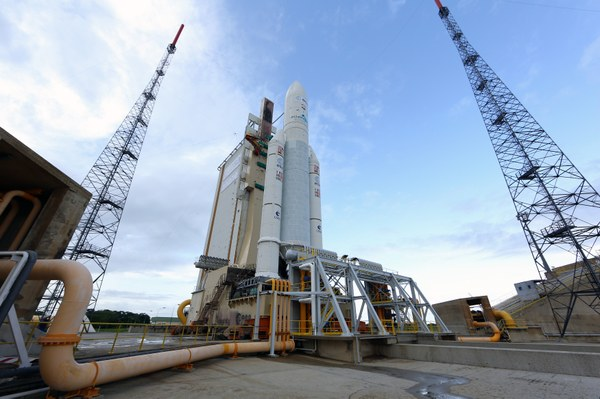
\includegraphics[width=\textwidth]{Bilder/ariane.jpeg}
		
		\column{0.25\textwidth}
		\centering
		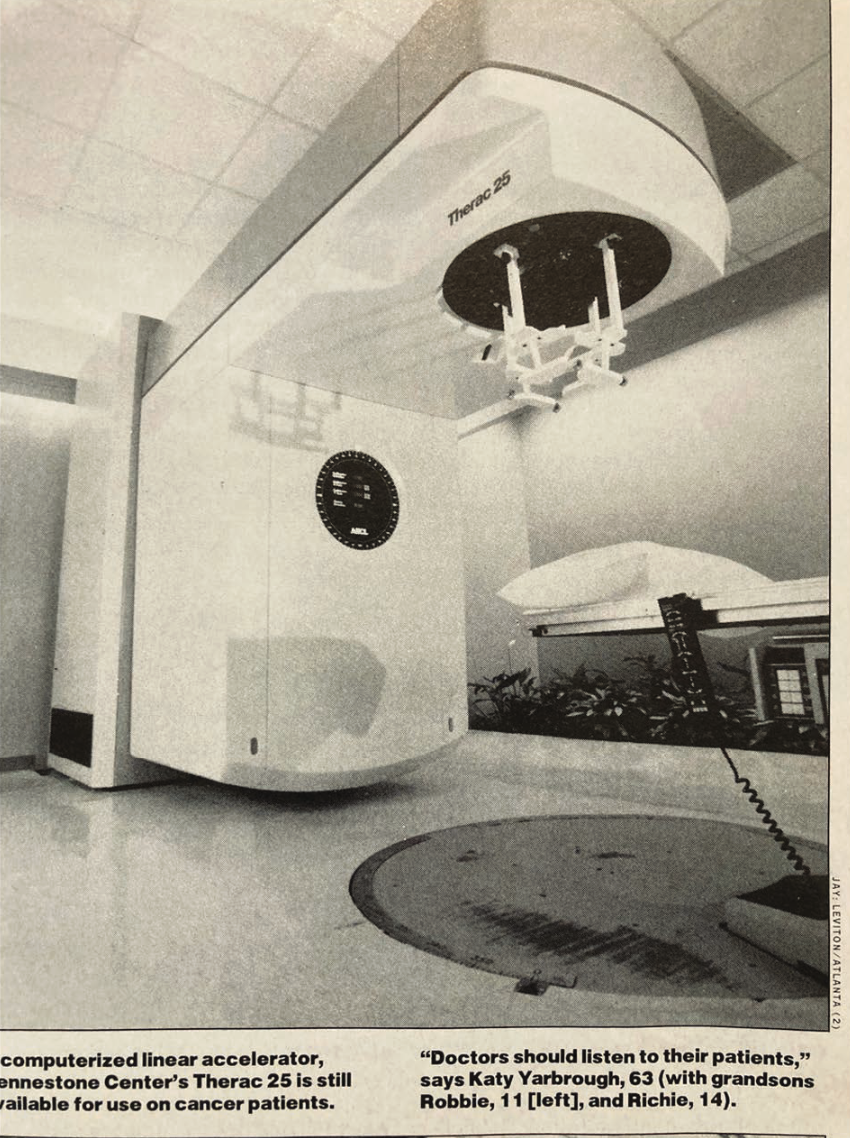
\includegraphics[width=\textwidth]{Bilder/therac.png}
	\end{columns}
	
	\vspace{0.2cm}
	
	\begin{center}
		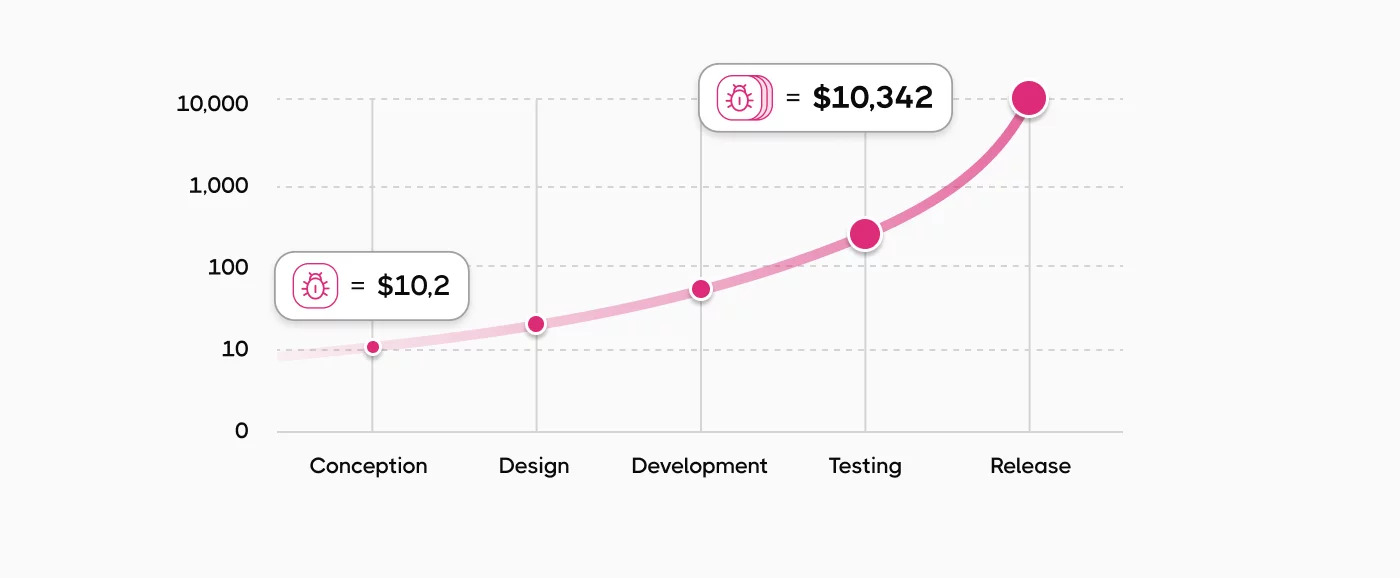
\includegraphics[width=0.7\textwidth]{Bilder/bugcost.jpg}
	\end{center}
	
\end{frame}
	
	
	\begingroup
	\tucthreeheadlines
	\title{Wie kann man formal korrekte SW schreiben}
	\frame{\titlepage}
	\endgroup
	
	\begingroup
	\tucthreeheadlines
	\title{Wie kann man formal korrekte SW schreiben*}
	\subtitle{*unter bestimmten Annahmen}
	\frame{\titlepage}
	\endgroup
	
	\frame{\tableofcontents}
	
	\newpage	
	\section{Methoden zur Sicherstellung von Codequalität}
	\begin{frame}
		\begin{center}
		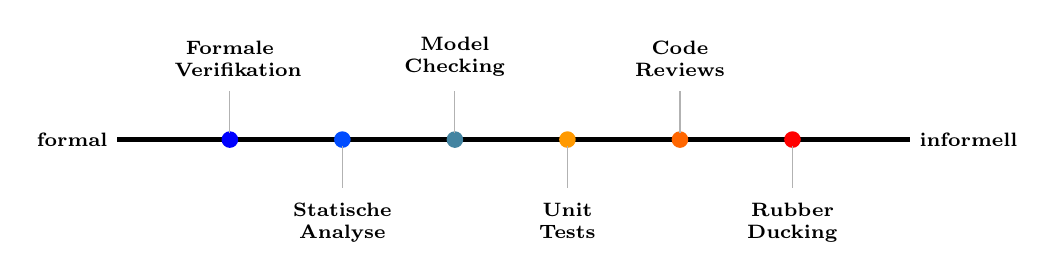
\begin{tikzpicture}[y=1cm, font=\scriptsize]
			
			% ------------------------------------------------------------
			% Positionen
			% ------------------------------------------------------------
			
			\def\xstart{0}
			\def\xend{0.83\textwidth}
			
			% Formal methods: deliberately close together
			\def\xformal{0.142*\xend}
			\def\xspec{2*0.142*\xend}
			\def\xstatic{3*0.142*\xend}
			
			% Less formal methods: more spacing
			\def\xreview{4*0.142*\xend}
			\def\xtest{5*0.142*\xend}
			\def\xmanual{6*0.142*\xend}
			
			% ------------------------------------------------------------
			% Axis labels
			% ------------------------------------------------------------
			
			\node[anchor=east] at (\xstart,0)
			{\textbf{formal}};
			
			\node[anchor=west] at (\xend,0)
			{\textbf{informell}};
			
			% ------------------------------------------------------------
			% Main axis
			% ------------------------------------------------------------
			
			\draw[line width=2pt, -, >=stealth]
			(\xstart,0) -- (\xend,0);
			
			% ------------------------------------------------------------
			% Markers
			% ------------------------------------------------------------
			
			\fill[blue]             (\xformal,0) circle (3pt);
			\fill[blue!70!cyan]     (\xspec,0)   circle (3pt);
			\fill[cyan!60!black]    (\xstatic,0) circle (3pt);
			\fill[orange!80!yellow] (\xreview,0) circle (3pt);
			\fill[orange!80!red]    (\xtest,0)   circle (3pt);
			\fill[red]              (\xmanual,0) circle (3pt);
			
			% ------------------------------------------------------------
			% Connecting lines
			% ------------------------------------------------------------
			
			\draw[gray!60]
			(\xformal,0.08) -- (\xformal,0.62);
			
			\draw[gray!60]
			(\xspec,-0.08) -- (\xspec,-0.62);
			
			\draw[gray!60]
			(\xstatic,0.08) -- (\xstatic,0.62);
			
			\draw[gray!60]
			(\xreview,-0.08) -- (\xreview,-0.62);
			
			\draw[gray!60]
			(\xtest,0.08) -- (\xtest,0.62);
			
			\draw[gray!60]
			(\xmanual,-0.08) -- (\xmanual,-0.62);
			
			% ------------------------------------------------------------
			% Labels
			% ------------------------------------------------------------
			
			\node[align=center, text width=1.4cm, anchor=south] at (\xformal,0.68)
			{\textbf{Formale\\Verifikation}};
			
			\node[align=center, text width=1.4cm, anchor=north] at (\xspec,-0.68)
			{\textbf{Statische\\Analyse}};
			
			\node[align=center, text width=1.5cm, anchor=south] at (\xstatic,0.68)
			{\textbf{Model\\Checking}};
			
			\node[align=center, text width=1.5cm, anchor=north] at (\xreview,-0.68)
			{\textbf{Unit\\Tests}};
			
			\node[align=center, text width=1.8cm, anchor=south] at (\xtest,0.68)
			{\textbf{Code\\Reviews}};
			
			\node[align=center, text width=1.5cm, anchor=north] at (\xmanual,-0.68)
			{\textbf{Rubber\\Ducking}};
		\end{tikzpicture}
		\end{center}
	\end{frame}
	
	%\begin{frame}
	%- woher weiß ich, dass mein Code das macht was er soll?
	%- formal(Korrektheitsbeweis, Pfadüberdeckung) vs informell(code-review...)
	%- computer gestützt?
	%\end{frame}
	
	\section{Passende Ansätze}
	\begin{frame}
	\begin{center}
		\begin{tikzpicture}[every node/.style={inner sep=0pt}]
			
			% ============================================================
			% Obere Reihe: Code -> formale Verifikation
			% ============================================================
			
			\node (python) at (0,2) {
				
\includegraphics[height=1.8cm]{Bilder/codeLogo.png}
			};
			
			\node (verification) at (5,2) {
				
\includegraphics[height=1.8cm]{Bilder/formalModel.jpeg}
			};
			
			\draw[->, >=stealth, line width=1.5pt]
			(python.east) -- (verification.west);
			
			\node[anchor=west, text width=4.5cm, align=left] at (6,2) {
				\textbf{}\\[-0.1cm]
				\begin{itemize}
					\item[\textcolor{green!50!black}{+}]
					Effizienter Code
					\item[\textcolor{red}{--}]
					Abstraktion komplex
				\end{itemize}
			};
				
				% ============================================================
				% Untere Reihe: Code <- formales Modell
				% ============================================================
				
				\node (model) at (0,-1.5) {
					
\includegraphics[height=1.8cm]{Bilder/codeLogo.png}
				};
				
				\node (code) at (5,-1.5) {
					
\includegraphics[height=1.8cm]{Bilder/formalModel.jpeg}
				};
				
				\draw[<-, >=stealth, line width=1.5pt]
				(model.east) -- (code.west);
				
				\node[anchor=west, text width=4.5cm, align=left] at (6,-1.5) {
					\textbf{}\\[-0.1cm]
					\begin{itemize}
						\item[\textcolor{green!50!black}{+}]
						Änderung des Models generiert neuen Code
						\item[\textcolor{red}{--}]
						Codegenerierung schwer steuerbar
					\end{itemize}
				};
				
		\end{tikzpicture}
	\end{center}	
	\end{frame}
	
	\section{Mein Ansatz}
	\begin{frame}
		\begin{figure}
			\centering
			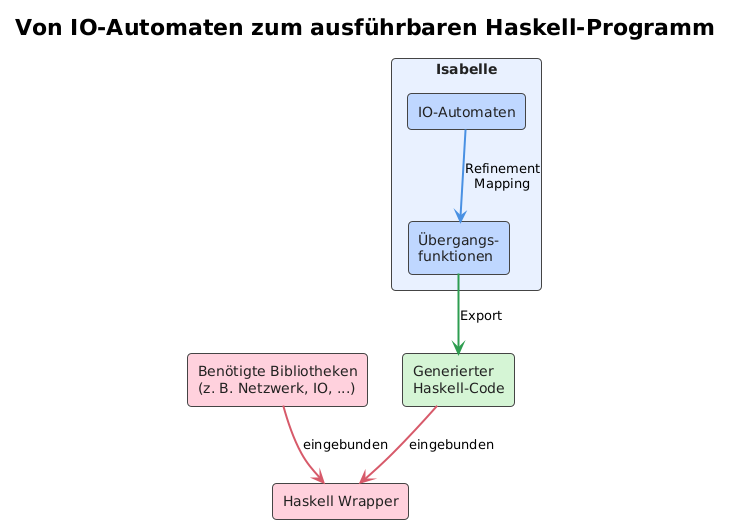
\includegraphics[height=\textheight]{Bilder/pipeline}
		\end{figure}
	\end{frame}
	\begin{frame}
	\begin{figure}
		\centering
		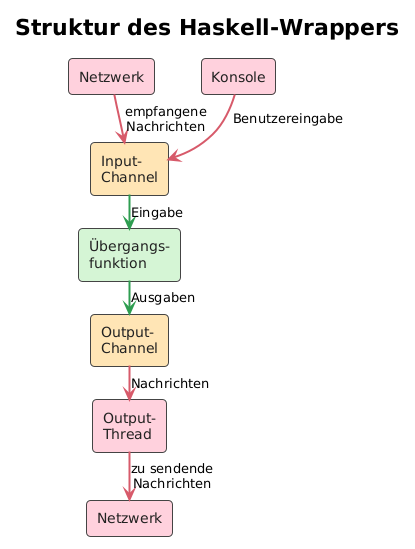
\includegraphics[height=\textheight]{Bilder/hswrapper}
	\end{figure}
	\end{frame}
	
	\section{Fazit}
	\begin{frame}
		\begin{itemize}
			\item[\textcolor{green!50!black}{+}]
			Haskell-Wrapper kann auf notwendiges IO-Mapping beschränkt werden
			\item[\textcolor{green!50!black}{+}]
			Beweise außerhalb von Isabelle auf ein Minimum reduziert
			\item[\textcolor{green!50!black}{+}]
			Eigentlicher Code erst nach der formalen Modellierung in Isabelle
			
			\item[\textcolor{red}{--}]
			Zusätzlicher Code durch Wrapper
			\item[\textcolor{red}{--}]
			Abhängigkeit von der Korrektheit des Codegenerators, Isabelle, verwendete Bibliotheken und Wrappers
			\item[\textcolor{red}{--}]
			Die Codegenerierung nur begrenzt steuerbar; generierte Code muss evtl. nachbearbeitet werden
		\end{itemize}
	\end{frame}
	
	\section*{Quellen}
	\begin{frame}
		\begin{itemize}
			\item \url{https://www.dlr.de/de/ar/themen-missionen/raumfahrttechnologien/traegersysteme/ariane-5} (3.9.26)
			\item \url{https://testomat.io/blog/software-bug-cost/} (3.9.26)
			\item \url{https://en.wikipedia.org/wiki/Therac-25} (3.9.26)
		\end{itemize}
	\end{frame}
\end{document}